\documentclass{article}

\usepackage{microtype}
\usepackage{graphicx}
\usepackage{subfigure}
\usepackage{booktabs}

\usepackage{hyperref}

\newcommand{\eat}[1]{}
\newcommand{\red}{\textcolor{red}}
\newcommand{\system}{\textsc{Krypton}}

\usepackage[accepted]{sysml2019}

\sysmltitlerunning{Demonstration of \textsc{Krypton}: Incremental and Approximate Inference for Faster Occlusion-based Deep CNN Explanations}

\begin{document}

\twocolumn[
\sysmltitle{Demonstration of \textsc{Krypton}: Incremental and Approximate Inference for Faster Occlusion-based Deep CNN Explanations}

\sysmlsetsymbol{equal}{*}

\begin{sysmlauthorlist}
\sysmlauthor{Supun Nakandala}{ucsd}
\sysmlauthor{Arun Kumar}{ucsd}
\end{sysmlauthorlist}

\sysmlaffiliation{ucsd}{University of California, San Diego}

\sysmlcorrespondingauthor{Supun Nakandala}{snakanda@eng.ucsd.edu}
% \sysmlcorrespondingauthor{Arun Kumar}{arunkk@eng.ucsd.edu}

\sysmlkeywords{Machine Learning, SysML}

\vskip 0.05in

\begin{abstract}
In this demonstration we present \system, a system for accelerating occlusion based deep convolution neural network (CNN) explainability workloads.
Driven by the success of CNNs in image understanding tasks, there is growing adoption of CNN technology in various domains including high stake applications such as radiology.
However, users of such applications often seek an ``explanation'' for why a CNN predicted a certain label.
One of the widely used approaches for explaining the CNN predictions is the occlusion based explainability (OBE) method.
This approach is computationally expensive due to the large number of re-inference requests produced.
In this demo we present \system~, a system that reduces the runtime of OBE by up to 35x by enabling incremental and approximate inference optimizations.
We allow the audience to interactively diagnose CNN predictions from several use cases including radiology and natural images.
\end{abstract}
]

\printAffiliationsAndNotice{} % otherwise use the standard text.

\vspace{-5mm}

\section{Introduction}\label{introduction}

Deep convolution neural networks (CNNs) are now the state of the art method for many image prediction tasks. Thus, there is growing interest in adopting deep CNNs in various application domains, including high stake applications such as radiology ~\cite{kermany2018identifying}.
Despite their successes, a key criticism of CNNs is that their internal workings are unintuitive to non-technical users. Thus, users often seek an ``explanation'' for why a CNN predicted a certain label.
How to explain a CNN prediction is still an active research question, but in the practical literature, an already popular mechanism for CNN explanations is a simple procedure called \textit{occlusion-based explanations}, or OBE for short.

OBE works as follows. Place a small patch (usually gray or black) on the image to occlude those pixels. Rerun CNN inference on the occluded image. The probability of the predicted label will change. Repeat this process by moving the patch across the image to obtain a sensitivity \textit{heat map} of the probability changes. This heat map will highlight regions of the image that were highly sensitive or ``responsible'' for the prediction (see red/orange color regions in Figure \ref{img:ui}). Such \textit{localization} of the regions of interest allows users to gain intuition on what ``mattered'' for the CNN prediction.

However, OBE is highly computationally expensive. Deep CNN inference is already expensive; OBE just amplifies it by issuing a large number of CNN re-inference requests. Such long wait times can hinder users' ability to consume explanations and reduce their productivity.

\begin{figure*}[t]\label{img:ui}
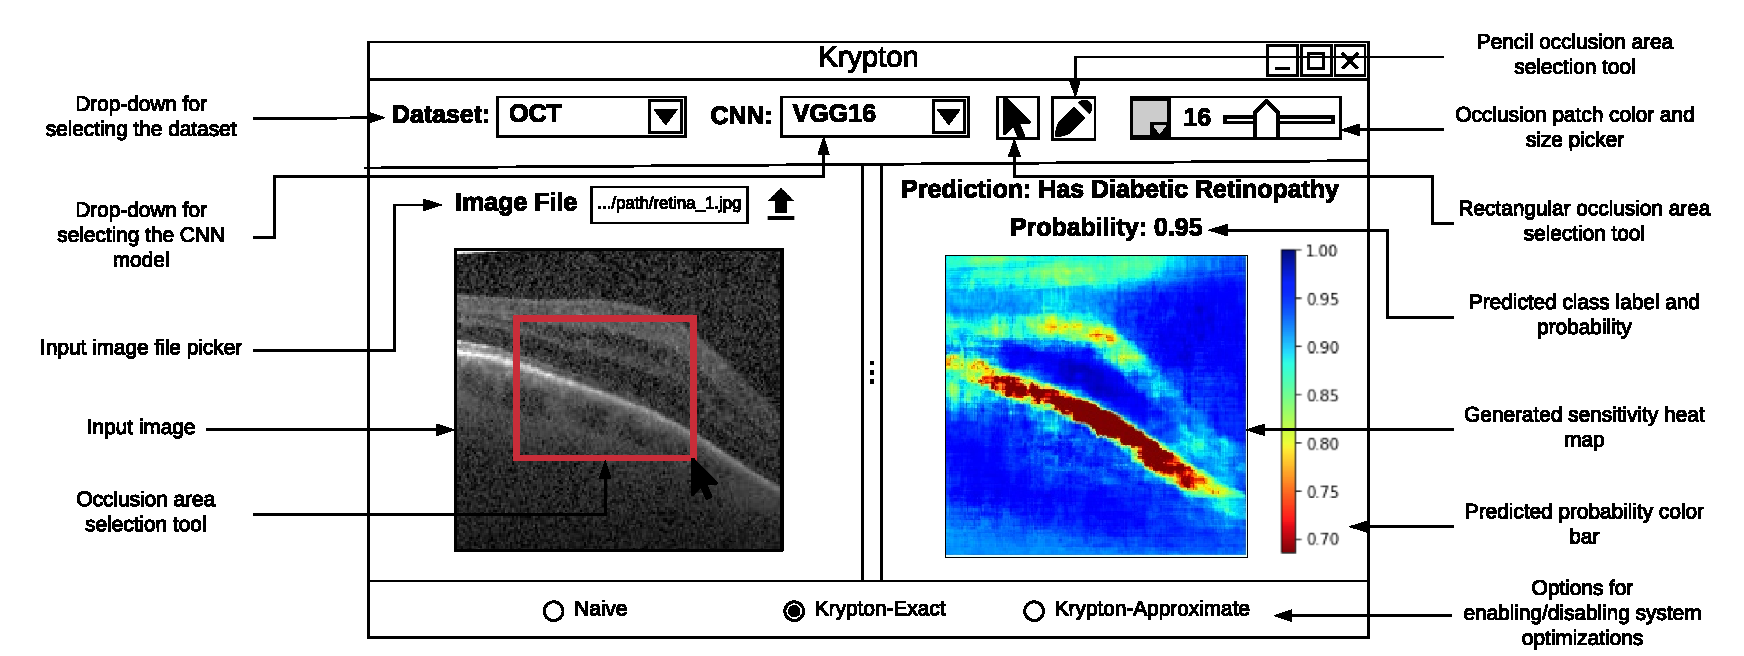
\includegraphics[width=\textwidth]{images/ui_mockup.pdf}
\vspace{-10mm}
\caption{\system~ user interface. Users can load an input image, select a CNN model and interactively diagnose the prediction by occluding parts of the image using brush or selection tool (left image). \system~ generates a sensitivity heat map (right image) and iteratively refines it as the user progresses.}
\vspace{-5mm}
\end{figure*}

\system~ uses a database-inspired lens to formalize, optimize, and accelerate OBE. We start with a simple but crucial observation: \textit{the occluded images are not disjoint but share most of their pixels; so, most of CNN re-inference computations are redundant.} Instead of treating a CNN as a ``blackbox,'' we open it up and formalize \textit{CNN layers} as ``queries.'' Just like how a relational query converts relations to other relations, a CNN layer converts \textit{tensors} (multidimensional arrays) to other tensors. So, we reimagine OBE as \textit{a set of tensor transformation queries} with incrementally updated inputs.

\system~ is implemented on top of popular deep learning framework PyTorch. It works on both CPU and GPU and currently supports a few popular deep CNNs. \system ~can enable up to $35$X speedups over the current dominant practice of running re-inference with just batching for producing high-quality approximate heat maps and up to $5$X speedups for producing exact heat maps.


\section{Technical Novelty}
The novelty of our system comes from the optimization techniques that it uses for accelerating the OBE workload.
Our first optimization is \textit{incremental CNN inference}. We \textit{materialize} all tensors produced by the CNN's layers on the given image. For every re-inference request in OBE, instead of rerunning CNN inference from scratch, we treat it as an incremental view maintenance (IVM) query, with the ``views'' being the tensors. We rewrite such queries to \textit{reuse} as much of the materialized views as possible and recompute only what is needed, thus \textit{avoiding computational redundancy}. Such rewrites are non-trivial because they are closely tied to the complex geometric dataflows of CNN layers. We have formalized such dataflows to create an \textit{algebraic framework} of CNN query rewrites. Going further, we batch all re-inference requests in OBE to reuse the \textit{same} materialized views. This is a form of multi-query optimization (MQO), albeit interwoven with our IVM, leading to a novel \textit{batched incremental CNN inference} procedure. To the best of our knowledge, this is the first instance of IVM being fused with MQO in query optimization, at least for CNN inference.

\system~ also performs two novel \textit{approximate inference} optimizations that allow users to tolerate some degradation in visual quality of the heat maps produced to reduce runtimes further. These optimizations build upon our incremental inference optimization to trade off heat map quality in a user-tunable manner. Our first approximate optimization, \textit{projective field thresholding}, draws upon an idea from neuroscience and exploits the internal semantics of how CNNs work. Our second approximate optimization, \textit{adaptive drill-down}, exploits the semantics of the OBE task and the way users typically consume the heat maps produced. We also present intuitive automated parameter tuning methods to help users adopt these optimizations.
More details on \system~ optimizations can be found in our Technical Report \cite{krypton}.


\section{Demonstration}\label{demonstration}
\textbf{Datasets and CNN models.} In this demonstration we will present an evaluation of \system ~with three real-world image datasets: 1) identifying diabetic retinopathy from retinal images, 2) identifying pneumonia from chest X-ray images, and 3) identifying objects from natural images in the ImageNet dataset. \system~ currently supports three popular CNN architectures, VGG, ResNet, and Inception models. Altogether, each participant will be able to interact with the system on nine different settings.

\textbf{Walkthrough.} Each participant will be first made familiar with OBE method and the \system~ system.
A participant will interact with the system using the user interface shown in Figure \ref{img:ui}.
First the participant will pick the dataset and the CNN model that they want to explore using the drop down menus.
Then the participant can select a particular image from the selected dataset that they want to diagnose using the image file picker. This will load the input image to the left pane of the user interface and also show the predicted label and the probability on the right pane.
For occluding the input image participants have two options. First one is to use the rectangular selection tool. The other option is to use the brush tool which will enable the participant to select an occlusion region in free form.
When selecting the brush tool participants also have the option of changing the brush size. For both tools users have to select the color of the occlusion patch using the color picker drop-down menu.
After selecting occlusion tool, participants can then interactively occlude parts of the input image, probably starting from the regions that they think contributes most to the prediction.
While the participant interactively updates the occluded region, \system~ will show the sensitivity heat map generated so far in the right side pane and will continue update it with incremental updates as the participant progresses.

\vspace{-4mm}

\bibliography{main.bib}
\bibliographystyle{sysml2019}
\end{document}
